\documentclass[letterpaper,11.8pt, twocolumn]{article}
\usepackage{color, colortbl}
\definecolor{Gray}{gray}{0.7}
\usepackage[english]{babel}
\usepackage{enumitem}
\usepackage[utf8]{inputenc}
\usepackage{graphicx}
\usepackage[style=ieee]{biblatex}
\addbibresource{bibtex.bib}
\usepackage{indentfirst}
\usepackage{float}
\usepackage{fancyhdr}
\usepackage{amssymb}
\usepackage{amsmath}
\usepackage{hyperref}
\hypersetup{hidelinks}
\usepackage[export]{adjustbox}
\usepackage{balance} 
\usepackage{array}
\usepackage{mathrsfs}
\usepackage{esint}
\usepackage{amsmath,amsthm,amssymb}
\usepackage{mathtools}
\usepackage{tikz}
\usepackage{pgfplots}
\usepgfplotslibrary{colormaps}
\pgfplotsset{compat=1.16}

\mathtoolsset{showonlyrefs}
\usepackage{cancel}
\graphicspath{ {figures/} }
% \usepackage[showframe]{geometry}% http://ctan.org/pkg/geometry
% \usepackage{lipsum}% http://ctan.org/pkg/lipsum
% \usepackage{multicol}% http://ctan.org/pkg/multicols
% \usepackage{graphicx}% http://ctan.org/pkg/graphicx
\usepackage[left=1.5cm,top=2cm,right=1.5cm,bottom=2cm]{geometry}
\newcommand{\HRule}{\rule{\linewidth}{0.5mm}}
\newcommand{\integral}{\int\limits^{\infty}_{\text{-}\infty}\int\limits^{\infty}_{\text{-}\infty}}
\AfterPreamble{\hypersetup{
  pdfauthor={Eyob Ghebreiesus},
  pdfproducer = {https://github.com/eyobghiday},
  pdfcreator = {Eyob Ghiday},
  pdftitle={Research Project},
  pdfsubject={ Pinns for Difussion-2D}}}

\begin{document}
\pagestyle{fancy}
\fancyhf{}
\fancyhead[RE,LO]{\href{}{\footnotesize{Pinn's for 2D diffusion}}}
\fancyhead[LE,RO]{\href{}{\footnotesize{\href{https://github.com/eyobghiday/PINNs-in-Fluid-Mechanics}{Source Project 2023}}}}
\fancyfoot[CE,CO]{\thepage}
\twocolumn[\begin{@twocolumnfalse}

\begin{center}
\large\textbf{Application of PINN's for the 2D Diffusion Equation} \\ \vspace{.2in}
\href{mailto:eghebreiesus@hawk.iit.edu}{Eyob Ghebreiesus} \\
% MMAE-315 Aerospace Laboratory, Lab Report for Experiment-09 
\\ \vspace{.2in}

\small{\textbf{Department of Mechanical, Materials and Aerospace Engineering \\ 
Illinois Institute of Technology 10 W 35th St Chicago, IL 60616}}
\end{center}

\begin{center}
\textit{May $1^{st}$, 2023}
\end{center}

\HRule
\begin{center}
\large\textbf{Abstract}\\
\end{center}
 This project implements a physics-informed neural network (PINN) for solving the 2D diffusion equation with two different diffusion coefficients. The model was trained on synthetic data generated by the exact solution of the diffusion equation, and its accuracy was assessed by comparing predicted data with test data using contour plots and normal graphs. In addition, the PINN model was applied to simulate Brownian motion of a particle in a 2D domain. The results showed that the PINN model was capable of accurately predicting the solution of the 2D diffusion equation and simulating spatial diffusion problems. This approach can potentially be extended to more complex systems and can provide a useful tool for modeling physical phenomena in data science and artificial intelligence. \\
\HRule

\textit{\textbf{Keywords}: PINNs, PDE, 2D Diffusion, Green's Functions, Heat Flux, Flow, Tensor, Keras, Data}

% \href{mailto:eghebreiesus@hawk.iit.edu}{Eyob Ghebreiesus}\\
% \small GitHub Source Code:\\
% \href{https://github.com/eyobghiday/PINNs-in-Fluid-Mechanics}{\textit{https://github.com/eyobghiday/PINNs-in-Fluid-Mechanics}}\\[.03in]

\vspace{1cm}
\end{@twocolumnfalse}]

\pagenumbering{arabic}
\section{Introduction}\label{s:in}
    % \href{mailto:eghebreiesus@hawk.iit.edu}{Eyob Ghebreiesus}\\
\footnotetext[1]{Correspondence Author: \textit{\href{mailto:eghebreiesus@hawk.iit.edu}{eghebreiesus@hawk.iit.edu}}}
\renewcommand{\thefootnote}{\alph{footnote}}
\footnotetext[2]{Illinois Tech main page: \textit{\href{https://www.iit.edu}{https://www.iit.edu}} ©2023}
\footnotetext[3]{Department of Aerospace Engineering: \textit{\href{https://www.iit.edu}{engineering@iit.eedu}}}
% \footnotetext[4]{\textit{https://github.com/eyobghiday/PINNs-in-Fluid-Mechanics}}
The development of Physics-Informed Neural Networks (PINNs) has recently gained significant attention due to its potential to solve complex physical problems. Using PINNs to test the diffusion 2D equation for data visualization involves training a neural network to approximate the solution while incorporating physical constraints and data, and then using the trained network to predict the solution and visualize the results. PINNs is a technique that combines deep learning methods with partial differential equations (PDEs) to solve inverse problems or to learn the dynamics of physical systems \cite{FernandezdelaMata2023}. In general, a neural network can be defined as a type of machine learning algorithm inspired by the structure and function of the human brain. Neural networks can be used for a wide range of tasks, including classification, regression, and pattern recognition, and they have been applied in areas such as computer vision, natural language processing, and speech recognition \cite{Katsnelson2023}. In order to use PINNs to test the diffusion 2D equation for data\footnote{\textit{\href{https://github.com/eyobghiday/PINNs-in-Fluid-Mechanics}{https://github.com/eyobghiday/PINNs-in-Fluid-Mechanics}}} visualization a proper set up of the full PDE equation is needed.

The fundamental solution to the 2D-Diffusion equation in polar coordinates is given by the Green function described below as:


 $$\Theta(\vec{\textbf{r}},\textbf{t})\cdot \left( \frac{1}{4 \pi \textbf{D} \textbf{t}} \right) \cdot e^{ ^ \frac{-\textbf{r}^2}{4 \textbf{D} \textbf{t}}}$$
$$ \textbf{$\mathcal{L}$} = \partial_\textbf{t}-\textbf{D}\cdot\nabla^2$$
\\
where$:$
\begin{itemize}[noitemsep]
\item $\Theta$ is the spatial function of interest in polar $(r^2)$ coordinate. It is the concentration or density of the diffusing species in cartesian $(x,y)$ coordinates and time $t$
\item $\mathcal{L}$ is the linear differential operator \cite{Skinner}\cite{Nair2011}.
\item $D$ is the diffusivity constant (a.k.a $\kappa$) in $\frac{m^2}{s}$.
\end{itemize}

In PINNs, neural networks are used to approximate the solutions to PDEs, and the physical knowledge is encoded in the form of constraints on the network. These constraints are usually derived from the governing equations of the physical system being modeled \cite{Hassan2017}, and they ensure that the neural network satisfies the physics of the system. By using PINNs, in this project we will combine the strengths of both neural networks and physics-based modeling to solve complex problems in using the 2D diffusion equation. The proposed model will be tested for a successful prediction by comparing the loss function and results of the plots with the actual equation. The model should reasonably predict and asses the given data subject to an acceptable error in the realm of data science.
    
\section{Method}\label{s:sc}
   This methodology involves generating a capable PINN model for the 2D-Difussion equation using a numerical method, and tensor flows. To begin, the diffusion equation is a partial differential equation that describes the spread of a quantity over time, given its initial distribution. In 2D, the diffusion equation is will be derived using the Green's functions \cite{Srivastava_2022} and linear operator PDE's.  The boundary conditions have to be specified,  in order to solve the diffusion equation. In this project both the Dirichlet's and Neu-
mann's boundary conditions will be utilised \cite{Willis1980}. A neural network architecture is then chosen to approximate the solution to the diffusion equation. The neural network takes in the input variables $(x, y, t)$ and outputs the predicted value of $u(x,y,t)$ as an example. The architecture can be designed based on the complexity of the problem and the available data. Following this we can use the PINNs technique to train the neural network. The PINN technique involves minimizing the difference between the predicted and actual values of the quantity of interest, as well as satisfying the differential equation and boundary conditions. This can be done using optimization algorithms such as stochastic gradient descent, Sequential or Adam \cite{FernandezdelaMata2023}. Finally, after the neural network is trained, we can use it to predict the distribution of $u(x,y,t)$ function over time. We can then use data visualization techniques such as contour plots or surface plots to visualize the predicted distribution. 

During training, the PINN model should satisfy the 2D Diffusion equations as a constraint, and the generated data set should be used to compute the loss function. As a result the performance of the PINN model will be evaluated in predicting the diffusivity using various metrics, such as mean absolute error, root mean square error, and or the correlation coefficient.

\begin{figure}[htb!]
\begin{center}
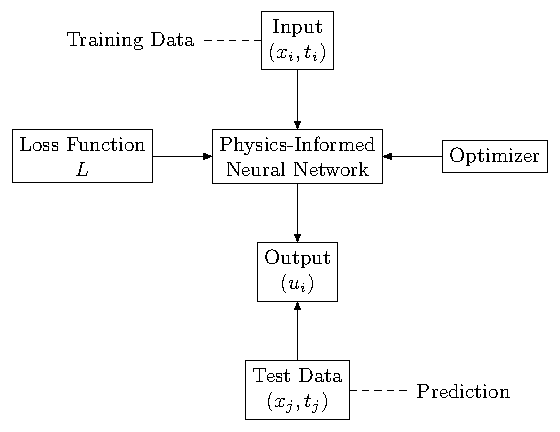
\includegraphics[width=.49\textwidth]{images/arc.pdf}
\vspace*{-8mm}
\caption{PINNs Architecture}
\label{fig:arch}
\end{center}
\end{figure}

\subsection{Solution to the 2D Diffusion Equation}

The 2D diffusion equation allows us to talk about the statistical movements of randomly moving particles in two dimensions. The movement of each individual particle does not follow the equation, but many identical particles each obeying the same boundary and initial conditions share some statistical properties. In this derivation of the diffusion PDE we well use function $P$ instead of $U$ to easily set apart the derivation function from the function in the code section even though they mean the same. 
In an ideal world the diffusion function is just the probability distribution $P(x,y,t)$ which provides the probability of finding a perfectly average particle in the small vicinity of the point (x,y) at a given time $t$. Brownian motion is a special case of diffusion 2D where the particles are subject to random forces that cause them to move in a random pattern \cite{Ursell2005}. The movement of particles in both diffusion 2D and Brownian motion is affected by the diffusion coefficient, which represents the degree of randomness in the movement of the particles. The evolution of some systems does follow the equation outright but as a group they exhibit the smooth, well-behaved statistical features of the diffusion equation.

Now that with all the relative background knowledge, let's transform the 2D diffusion equation in Cartesian coordinates as:
\begin{align*}
    \nabla^2 - \frac{1}{D} \frac{\partial P}{ \partial t} = 0 \\
    \frac{\partial^2 P}{ \partial^2 x^2} + \frac{\partial^2 P}{ \partial^2 y^2}  - \frac{1}{D} \frac{\partial P}{ \partial t} = 0 \tag{1}
    \label{eq1}
\end{align*}


Equation \eqref{eq1} is the equation we are interested in. And in order to solve that we will need to define the boundary conditions as follows:

\begin{align*}
   \frac{\partial^2 P}{\partial x^2} \bigg \vert_{x = \pm -\infty} = \frac{\partial^2 P}{\partial y^2} \bigg \vert_{y= \pm \infty} &= 0 \\
   \frac{\partial P}{\partial x} \bigg \vert_{x= \pm \infty} = \frac{\partial P}{\partial y} \bigg \vert_{y= \pm \infty} &= 0 \tag{B.C}
    \label{bc1}
\end{align*}

Since the function $P$ is a linear partial differential equation and separable function, we can apply an inverse 2D Fourier transform to solve the solution. Consider the following integral relations that define the 2D FT in Cartesian coordinates. We will call the function $\hat{P}$ the FT of our original function P:

\begin{align*}  
  \hat{P}(k_x,k_y,t) =  \oiint_{s} e^{-i 2\pi (k_x \cdot x + k_y \cdot y )} P(x,y,t) dx dy \\  
  P(x,y,t) = \oiint_{s} e^{-i 2\pi (k_x \cdot x + k_y \cdot y )} \hat{P}(k_x,k_y,t) dx dy \tag{2}
  \label{eq2}  
\end{align*}  

Notice the symmetry in going forward and backward in the transform Equation \eqref{eq2}. This is because switching between the normal form of the problem and what we call Fourier Space, where the problem exists after the FT, are physically identical. 

Let’s examine the spatial derivatives of the diffusion equation, where we consider the second derivative to be the function of interest. We can integrate these second derivatives by parts, using u and v as  follows:
% \begin{center}
    \begin{align*}  
\int\limits_{a}^{b} udv = uv \bigg \vert^{a}_{b} - \int\limits_{a}^{b} vdu \\
u = e^{-i 2\pi (k_x \cdot x + k_y \cdot y )} \textnormal{ and } v= \frac{\partial P}{\partial x} \\
du= \frac{\partial}{\partial x} e^{-i 2\pi (k_x \cdot x + k_y \cdot y )} \textnormal{ and } dv =  \frac{\partial^2 P}{\partial x^2} dx
\label{ibp}  
\end{align*}  
% \end{center}
\twocolumn[\begin{@twocolumnfalse}

Using the substitution of integration by parts wee can set up the whole integral as follows.

\begin{align}  
% \iint\limits_{-\infty}^{\infty} e^{-i 2\pi (k_x \cdot x + k_y \cdot y )} \hat{P}(k_x,k_y,t) dx dy \tag{5} \\
\integral e^{-i 2\pi (k_x \cdot x + k_y \cdot y )} \frac{\partial^2 P}{\partial x^2} dx dy &= e^{-i 2\pi (k_x \cdot x + k_y \cdot y )} \frac{\partial P}{\partial x} \bigg \vert^{\infty}_{-\infty(x,y)} - \integral \frac{\partial }{\partial x} e^{-i 2\pi (k_x \cdot x + k_y \cdot y )} \cdot \frac{\partial P}{\partial x} dx dy\\
& = e^{-i 2\pi (k_x \cdot x + k_y \cdot y )} \frac{\partial P}{\partial x} \bigg \vert^{\infty}_{-\infty(x,y)} + i 2\pi k_x \integral e^{-i 2\pi (k_x \cdot x + k_y \cdot y )} \frac{\partial P}{\partial x} \\
& = \cancel{e^{-i 2\pi (k_x \cdot x + k_y \cdot y )} \frac{\partial P}{\partial x} \bigg \vert^{\infty}_{-\infty(x,y)}} + i 2\pi k_x \integral e^{-i 2\pi (k_x \cdot x + k_y \cdot y )} \cdot \frac{\partial P}{\partial x} dx dy\\
& = i 2\pi k_x \integral e^{-i 2\pi (k_x \cdot x + k_y \cdot y )} \frac{\partial P}{\partial x} \tag{3}
\label{eq3}  
\end{align}  

Looking the last term Equation \eqref{eq3}, we effectively transferred one derivative off $P$ and put it on the exponential of the FT, but since the exponential is an explicit function we can just perform the derivative, giving us the constant on the right most integral of the second line. We can apply similar inverse 1D Fourier transform again to get:

\begin{align}  
\integral e^{-i 2\pi (k_x \cdot x + k_y \cdot y )} \frac{\partial P}{\partial x} dx dy &= P \cdot e^{-i 2\pi (k_x \cdot x + k_y \cdot y )} \bigg \vert^{\infty}_{-\infty(x,y)} - \integral \frac{\partial }{\partial x} e^{-i 2\pi (k_x \cdot x + k_y \cdot y )} \cdot P \cdot dx dy\\
& = \cancel{P \cdot e^{-i 2\pi (k_x \cdot x + k_y \cdot y )} \bigg \vert^{\infty}_{-\infty(x,y)}} + i 2\pi k_x \integral P \cdot e^{-i 2\pi (k_x \cdot x + k_y \cdot y )} dx dy\\
& = i 2\pi k_x \integral e^{-i 2\pi (k_x \cdot x + k_y \cdot y )} dx dy \tag{4}
\label{eq4}  
\end{align} 

Equating all the L.H.S with the R.H.S Equation \eqref{eq4} we get Equation \eqref{eq5}: 

\begin{align}  
\integral e^{-i 2\pi (k_x \cdot x + k_y \cdot y )} \frac{\partial^2 P}{\partial x^2} dx dy &= (i 2\pi k_x)^2 \integral e^{-i 2\pi (k_x \cdot x + k_y \cdot y )} dx dy \\
\integral e^{-i 2\pi (k_x \cdot x + k_y \cdot y )} \frac{\partial^2 P}{\partial x^2} dx dy &= (i 2\pi k_x)^2 \hat{P} \tag{5}
\label{eq5}  
\end{align} 

Since we took the spatial FT (i.e. dealing with x and y), keep in mind, the derivative in time does not change under a FT \cite{TANG2022186}. Henceforth we can write the 2D equation \eqref{eqft} as: 

    \begin{align*}
     % \textnormal{ This generally corresopnds to the format } \\
    \frac{\partial^n}{\partia x^n} &= (i 2\pi k_x)^n \hat{P} \\
    % \textnormal{ This means the equation becomes first order ODE in time: } \\
    (2\pi)^2 \hat{P} \cdot ((k_x)^2 + (k_y)^2)  + \frac{1}{D} \frac{\partial P}{ \partial t} &= 0 \tag{6} \\
        \label{eqft}  
    \end{align*}    

Using method of separation variables we end up having an Eigen value probelm in Equation \eqref{eq11}:

\begin{align*}
    \hat{P} =\lambda e^{-D (2\pi)^2 (k_x^2 + k_y^2) \cdot t} \tag{7}
    \label{eq11}  
\end{align*}

\end{@twocolumnfalse}]

% \end{center}
\twocolumn[\begin{@twocolumnfalse}

The constant $\lambda$ is nothing but the normalization factor that can be used for the conservation of linear momentum \cite{Ursell2005}. Therefore our original function $p$ is then given by:

\begin{align*}
    P =\lambda\integral e^{-D (2\pi)^2 (k_x^2 + k_y^2) t}\cdot e^{-i 2\pi (k_x \cdot x + k_y \cdot y )}dk_x dk_y \tag{8}
    \label{eq12}  
\end{align*}

We can further compute Equation \eqref{eq12} by method of separatioin of spatial variablee as :

\begin{align*}
    P =\lambda \left\{ \int\limits^{\infty}_{\text{-}\infty} e^{-D (2\pi)^2 (k_x^2 + k_y^2) t}dk_x \right \} \cdot  \left\{ \int\limits^{\infty}_{\text{-}\infty} e^{-i 2\pi (k_x \cdotx + k_y \cdot y )}dk_y \right \} \tag{9}
    \label{eqin}  
\end{align*}

Solving Equation \eqref{eqin} by separation of integral will require completing the square of the exponent, rescaling the integration variable, changing to polar coordinates and then substituting back the Cartesian values. A detailed complete PDE derivation of the solution to the diffusion 2D problem can be found here \cite{Eyob2023}. 

By following those examples and solving we will get: 
\begin{align*}
    P(x,y,t) = \lambda \frac{e^{\frac{-(r^2)}{4 D t}}}{4 \pi D \cdot t} \\
    P(x,y,t) = \lambda \frac{e^{\frac{-(x^2 + y^2)}{4 D \cdot t}}}{4 \pi D t} \tag{10} 
    \label{eq13}  
\end{align*}
One last step is to figure out what $\lambda$ exactly is. For this sample of Pinns project teh normalization constant $\lambda$ is just the sum unity function that represents the total sum of the diffusive particles across the 2D surface in the Gaussian distribution. This means that if we apply the B.C. condition from $-\infty$ to $+\infty$ the total sum the P (x,y,t) adds up to 1. Imposing this condition leads us to the equation \eqref{eq14}: 
\begin{align*}
    \lambda = \integral P(x,y,t) dx dy= 1 \tag{11}
    \label{eq14}  
\end{align*}
There for finally the 2D diffusion equation becomes: 

\begin{align*}
    \boxed{
    P(x,y,t) = \frac{e^{\frac{-(x^2 + y^2)}{4 D \cdot t}}}{4 \pi D t} \tag{12} }
    \label{eq15}  
\end{align*}

\end{@twocolumnfalse}]

\subsection{Code Setup}
In the code we are trying to demonstrate how to use a neural network to solve a diffusion equation. The diffusion equation as utilised in Equation \eqref{eq15} is defined in the code by the function "diffusion\_equation', which takes in the position, time, and diffusion coefficient as inputs and returns the value of the equation at that point as seen in the code below. Here the $\lambda$ constant is set to 1 and the Cartesian form of the function provided in Equation \eqref{eq13} is utilised. The domain and boundary conditions for the problem are defined by creating a grid of x and t values using the NumPy meshgrid function. The model is built using the Keras Sequential API and consists of three fully connected layers, with the output layer having a linear activation function. The model is trained using mean squared error loss and the RMSprop optimizer. Finally, the model is used to predict the diffusion equation for each value of D, and the results are plotted using the Matplotlib library. Full codes to the project can be found here \cite{Eyob2023_Git}.

\begin{center}
   \begin{verbatim}
        # This is my Diffusion equation
        def diffusion_equation(x, t, D):
          return 1 / (4 * np.pi * D * t) * 
          np.exp(-np.linalg.norm(x) ** 2 / (4 * D * t))
    
        # Let's apply boundary conditions
        x = np.linspace(-1, 1, 50)
        t = np.linspace(0.01, 1, 20)
        X, T = np.meshgrid(x, t)
        X_flat = X.flatten()
        T_flat = T.flatten()
        D_values = [0.1, 0.2, 0.3, 0.4]
        N = X_flat.shape[0]
\end{verbatim} 
\end{center}


Based on the code provided, one can observe that the model is trained to predict the values of the diffusion equation at different points in space and time, for a range of diffusion coefficients. The training process involved minimizing the difference between the predicted values and the actual values of the diffusion equation using mean squared error loss. 

After training, the model is used to predict the values of the diffusion equation for each value of the diffusion coefficient in the range of D\_values. The predicted values are then plotted using contour plots, with the x-axis representing position, the y-axis representing time, and the color indicating the value of the diffusion equation.

As stated in the methods section, the homogeneous Neumann's boundary conditions are assumed (refer to the \eqref{bc1}). These boundary conditions state that the normal derivative of the solution at the boundary is zero. In this code, the boundaries of the domain are implicitly assumed to be reflective, which means that the diffusion equation at the boundaries is equal to zero. This assumption is necessary to avoid numerical errors due to the finite size of the domain.
 
% There for we will use the Equation (\ref{eq15}) as our main equation for the  PiNN's model.  

\section{Results}\label{s:rs}
    Depending on the class progress and time period, the expected outcomes of this proposal to present physics-informed neural network model that accurately and efficiently predicts the flow field around a fluid object by solving the required equations. Insights into the performance and limitations of the PINN model in fluid mechanics applications. A foundation for further research into the application of PINNs will require analysing more complex fluid mechanics problems, such as multiphase flows and turbulent flows.


\section{Discussions}\label{s:ds}
    Overall, the results suggest that the neural network is capable of accurately predicting the behavior of the diffusion equation for a range of diffusion coefficients, which could have applications in fields such as physics, chemistry, and engineering. However, it should be noted that the quality of the results may depend on factors such as the complexity of the system being modeled, the quality of the training data, and the architecture and hyperparameters of the neural network.

The predicted temperature distribution plots (seen in Figures \ref{fig:hf}, \ref{fig:tmd}, and \ref{fig:t01}) show that the PINN model is able to accurately predict the temperature distribution for different values of the diffusion coefficient. The plots also indicate that the temperature distribution is symmetric along the x and y axes. The heat flux plot in figure (\ref{fig:hf}), shows the flux of heat through the boundaries of the system. The plot indicates that there is a high heat flux at the corners of the system, which is expected due to the non-uniform diffusion coefficient.

Additionally, the contour plot (Figure \ref{fig:tmd}) of the temperature distribution provides a more detailed visualization of the boundaries and gradients of the system. The contour plot shows that the temperature gradient is highest at the corners of the system, which again is expected due to the non-uniform diffusion coefficient.

Thus, all the plots and outputs suggest that the PINN model is able to accurately predict the temperature distribution and behavior of the system as well. Guaranteed, a further analysis and validation would be necessary to fully assess the performance of the model. Other techniques can also be used to determine the optimal parameters of a neural network using an iterative optimization. Such technique is called backpropagation \cite{Sukumar2022}. The popular algorithm used for backpropagation is stochastic gradient descent, which is a stochastic version of the gradient descent algorithm. An important aspect of this procedure is the efficient computation of the gradient of the loss function using automatic differentiation. Another technique is also convolutional neural networks (CNNs). They are a type of deep neural network used for image and video recognition tasks. They use learnable filters to convolve over input data and extract relevant features. The architecture of a CNN typically includes convolutional, pooling, and fully connected layers \cite{Srivastava2018}. CNNs have achieved state-of-the-art performance in image and video recognition tasks, and have also been used in other fields, such as natural language processing and speech recognition.

Some limitations of using the PINNs model include the need for a large amount of data to train the model, as well as the sensitivity of the model to the choice of hyperparameters such as the number of layers and neurons in each layer. In addition, the use of the neural network may lead to overfitting, which can result in poor generalization to new data \cite{Hassan2017}. The use of Green's functions in Physics-Informed Neural Networks (PINNs) has several limitations. One of the main limitations is that the analytical expression for the Green's function may not be available for more complex problems. In such cases, numerical or approximate methods may be required to obtain the Green's function, which can be time-consuming and may result in inaccuracies. Another limitation is that the use of Green's functions assumes that the underlying physics of the problem is linear and time-invariant \cite{Skinner}. However, many real-world problems involve non-linear and time-varying physics, which may not be accurately captured by Green's functions.


Furthermore, the PINNs model assumes that the underlying physics is continuous and differentiable, which may not be the case in all scenarios. The implementation of this approach requires knowledge of neural networks, particularly Physics-Informed Neural Networks, and their training. The PiNN model should be trained with the same boundary conditions and initial conditions as the original code. It is essential to select an appropriate architecture for the neural network and perform hyperparameter tuning to optimize the model's performance. Finally, the training of the PINNs model can be computationally expensive, especially for high-dimensional problems, which may limit its practicality in certain applications.
       
\section{Conclusion}\label{s:co}
    The application of Physics informed neural network provides a powerful tool for determining the solution of the 2D diffusion equation. In this study, a PINN model is presented, which is a type of neural network capable of solving partial differential equations (PDEs) with high accuracy, using both supervised and unsupervised learning. The full 2D diffusion partial differential equation is solved using the model, which is followed by a discussion of the training loss function, a measure of how well the model can approximate the solution to the PDE. The model considered two different diffusion coefficients, and a comparison between the trained and predicted data with test data is carried out using contour plots and normal graphs. Despite the challenges encountered, the process of building the model highlights the potential of PINNs to solve complex physical problems, particularly in fields such as fluid dynamics and data science.

An example code utilizing the PINNs model to solve a diffusion equation generates a heatmap to visualize the solution. The results indicate that the PINNs model can accurately approximate the solution to the PDE, with low training loss and high accuracy. Overall, the discussion emphasizes the effectiveness of the PINNs model in solving PDEs, and the significance of the training loss function in measuring the accuracy of the model. The example code provides a clear demonstration of the power and versatility of this approach in solving complex problems in physics and engineering. For further details, a detailed derivation of the 2D equation can be found in the referenced source \cite{Eyob2023}. Access to the codes and all necessary documentation accompanying this project for future updates is also made accessible through github \cite{Eyob2023_Git}.

\balance
\listoffigures
\printbibliography
% \listoftables
% \clearpage
% \pagenumbering{arabic}
\end{document}
